












%%%%%%%%%%%%%%%%%%%%%%%%%%%%%%%%%%%%%%%%%
% Beamer Presentation
% LaTeX Template
% Version 1.0 (10/11/12)
%
% This template has been downloaded from:
% http://www.LaTeXTemplates.com
%
% License:
% CC BY-NC-SA 3.0 (http://creativecommons.org/licenses/by-nc-sa/3.0/)
%
%%%%%%%%%%%%%%%%%%%%%%%%%%%%%%%%%%%%%%%%%

%----------------------------------------------------------------------------------------
%	PACKAGES AND THEMES
%----------------------------------------------------------------------------------------

\documentclass[unicode]{beamer}

\mode<presentation> {

% The Beamer class comes with a number of default slide themes
% which change the colors and layouts of slides. Below this is a list
% of all the themes, uncomment each in turn to see what they look like.

%\usetheme{default}
%\usetheme{AnnArbor}
%\usetheme{Antibes}
%\usetheme{Bergen}
%\usetheme{Berkeley}
%\usetheme{Berlin}
%\usetheme{Boadilla}
%\usetheme{CambridgeUS}
%\usetheme{Copenhagen}
%\usetheme{Darmstadt}
%\usetheme{Dresden}
%\usetheme{Frankfurt}
%\usetheme{Goettingen}
%\usetheme{Hannover}
%\usetheme{Ilmenau}
%\usetheme{JuanLesPins}
%\usetheme{Luebeck}
\usetheme{Madrid}
%\usetheme{Malmoe}
%\usetheme{Marburg}
%\usetheme{Montpellier}
%\usetheme{PaloAlto}
%\usetheme{Pittsburgh}
%\usetheme{Rochester}
%\usetheme{Singapore}
%\usetheme{Szeged}
%\usetheme{Warsaw}

% As well as themes, the Beamer class has a number of color themes
% for any slide theme. Uncomment each of these in turn to see how it
% changes the colors of your current slide theme.

%\usecolortheme{albatross}
%\usecolortheme{beaver}
%\usecolortheme{beetle}
%\usecolortheme{crane}
%\usecolortheme{dolphin}
%\usecolortheme{dove}
%\usecolortheme{fly}
%\usecolortheme{lily}
%\usecolortheme{orchid}
%\usecolortheme{rose}
%\usecolortheme{seagull}
%\usecolortheme{seahorse}
%\usecolortheme{whale}
%\usecolortheme{wolverine}

%\setbeamertemplate{footline} % To remove the footer line in all slides uncomment this line
%\setbeamertemplate{footline}[page number] % To replace the footer line in all slides with a simple slide count uncomment this line

%\setbeamertemplate{navigation symbols}{} % To remove the navigation symbols from the bottom of all slides uncomment this line
}

\usepackage[utf8]{inputenc}
\usepackage[english, russian]{babel}
\usepackage{cmap}

\usepackage{verbatim}
\usepackage{fancybox}
\usepackage{ulem}
\usepackage{tikz}
\usetikzlibrary{positioning}
\usepackage{scalefnt}
\usetikzlibrary{arrows,shapes,positioning,shadows,trees,calc,backgrounds,fit,positioning}

\usepackage{graphicx} % Allows including images
\usepackage{booktabs} % Allows the use of \toprule, \midrule and \bottomrule in tables
\usepackage{textcomp}
\usepackage{listings}
\usepackage{color}
\usepackage{xcolor}
\usepackage{changepage}
\usepackage{pbox}

\tikzset{
  basic/.style  = {draw, text width=2cm, drop shadow, font=\sffamily, rectangle},
%  root/.style   = {basic, rounded corners=2pt, thin, align=center,
%                   fill=green!60},
  level 2/.style = {basic, rounded corners=6pt, thin, align=center, fill=green!60,
                   text width=7em},
  level 3/.style = {basic, thin, align=left, fill=pink!60, text width=6.5em}
}

\definecolor{mygreen}{rgb}{0,0.6,0}
\definecolor{mygray}{rgb}{0.5,0.5,0.5}
\definecolor{mymauve}{rgb}{0.58,0,0.82}

\lstset{ %
  backgroundcolor=\color{white},   % choose the background color; you must add \usepackage{color} or \usepackage{xcolor}
  basicstyle=\footnotesize,        % the size of the fonts that are used for the code
  breakatwhitespace=false,         % sets if automatic breaks should only happen at whitespace
  breaklines=true,                 % sets automatic line breaking
  captionpos=b,                    % sets the caption-position to bottom
  commentstyle=\color{mygreen},    % comment style
  deletekeywords={...},            % if you want to delete keywords from the given language
  escapeinside={\%*}{*)},          % if you want to add LaTeX within your code
  extendedchars=true,              % lets you use non-ASCII characters; for 8-bits encodings only, does not work with UTF-8
  frame=single,                    % adds a frame around the code
  keepspaces=true,                 % keeps spaces in text, useful for keeping indentation of code (possibly needs columns=flexible)
  keywordstyle=\color{blue},       % keyword style
  language=Octave,                 % the language of the code
  morekeywords={*,...},            % if you want to add more keywords to the set
  numbers=left,                    % where to put the line-numbers; possible values are (none, left, right)
  numbersep=5pt,                   % how far the line-numbers are from the code
  numberstyle=\tiny\color{mygray}, % the style that is used for the line-numbers
  rulecolor=\color{black},         % if not set, the frame-color may be changed on line-breaks within not-black text (e.g. comments (green here))
  showspaces=false,                % show spaces everywhere adding particular underscores; it overrides 'showstringspaces'
  showstringspaces=false,          % underline spaces within strings only
  showtabs=true,                  % show tabs within strings adding particular underscores
  stepnumber=1,                    % the step between two line-numbers. If it's 1, each line will be numbered
  stringstyle=\color{mymauve},     % string literal style
  tabsize=4,                       % sets default tabsize to 2 spaces
  %title=\lstname                   % show the filename of files included with \lstinputlisting; also try caption instead of title
}

\graphicspath{{./figures/}}

%----------------------------------------------------------------------------------------
%	TITLE PAGE
%----------------------------------------------------------------------------------------

\title[Обработка и исполнение запросов: лекция 11]{Обработка и исполнение запросов в СУБД \\~\\ (Лекция 11) \\~\\ Физический дизайн в СУБД\\~\\ v3} % The short title appears at the bottom of every slide, the full title is only on the title page

\author{Георгий Чернышев} % Your name
\institute[ВШЭ] % Your institution as it will appear on the bottom of every slide, may be shorthand to save space
{
Высшая Школа Экономики \\ % Your institution for the title page
\medskip
\textit{chernishev@gmail.com} % Your email address
}
\date{9 декабря 2020 г.} % Date, can be changed to a custom date

\begin{document}

\begin{frame}
\titlepage % Print the title page as the first slide
\end{frame}

\begin{comment}
\begin{frame}
\frametitle{Overview} % Table of contents slide, comment this block out to remove it
\tableofcontents % Throughout your presentation, if you choose to use \section{} and \subsection{} commands, these will automatically be printed on this slide as an overview of your presentation
\end{frame}
\end{comment}

\section{Введение}

%\subsection{???}

\begin{frame}
\frametitle{План}
{\scriptsize
\begin{itemize}
  \item Задача настройки СУБД.
  \begin{itemize}
    \item Автоматическая настройка СУБД;
    \item Физические структуры и что можно получить;
    \item Формальная постановка, решение.   
  \end{itemize}
  \item ``Классификация'' методов решения на примере задачи верт. фрагментирования:
  \begin{itemize}
    \item процедурные;
    \item стоимостные;
    \item смешанные;
  \end{itemize}  
  \item Горизонтальное фрагментирование:
  \begin{itemize}
    \item типы с точки зрения пользователя;
    \item фрагментирование на основе предикатов;
    \item распространение по ключам;
  \end{itemize} 
  \item Размещение данных
  \begin{itemize}
    \item Цели
    \item Типы: классификация по объекту размещения и избыточности;
    \item Размещение и фрагментирование;
    \item Модели в задаче размещения;
    \item Динамическая постановка;
  \end{itemize} 
  \item Современные работы.
  
\end{itemize}
}
\end{frame}

\begin{frame}
\frametitle{Задача настройки СУБД (1)}
Задача настройки СУБД под известную схему данных и известный набор запросов~--- одна из самых старых задач области баз данных.\\~\\

Успешное решение позволяет существенно повысить производительность СУБД или добиться нужных значений других необходимых характеристик.\\~\\

\end{frame}

\begin{frame}
\frametitle{Задача настройки СУБД (2)}

Администратор баз данных может:
\begin{itemize}
  \setlength\itemsep{1em}  
  \item переписать запросы, расставить подсказки или иным образом повлиять на план выполнения \alert{конкретного} запроса;
  \item изменить параметры СУБД (используемый размер оперативной памяти, максимальное количество соединений к базе, политики журналирования и прочее);
  \begin{itemize}
  	\item Пример: параметр $work\_mem$ в PostgreSQL задает максимально допустимый объем оперативной памяти, используемый в том числе для сортировки. Если данные не влезут~--- будет использоваться внешняя сортировка, со свопом на диск.
  \end{itemize}
  \item \alert{выбрать наиболее подходящие структуры физического уровня.}
\end{itemize}


Это делали (и делают) вручную, однако с момента появления области баз данных постоянно предпринимались попытки автоматизации.

\end{frame}


\begin{frame}
\frametitle{Задача автоматической настройки СУБД (1)}

Самые ранние работы по автоматизации выбора физических структур, что мне удалось найти: 
\begin{itemize}
  \setlength\itemsep{1em}
  \item в базах данных (задача вертикального фрагментирования): $\sim 1975$ год \cite{p1};
  \item задача о размещении файла в компьютерных сетях: $\sim 1969$ год \cite{p2};
  \item задача о снабжении военных складов: \\ $\sim 1940$ годы;
  \item ... дальше в прошлое не заглядывал, поэтому могут найтись еще предшественники!
\end{itemize}

\end{frame}

\begin{frame}
\frametitle{Задача автоматической настройки СУБД (2)}

Несмотря на зрелость, этот род задач до сих пор актуален:

\begin{itemize}
  \setlength\itemsep{1em}	
  \item Востребованность решения~--- индустрия заинтересована в качественных решениях, они дают экономический эффект;
  \item $NP$-трудность подавляющего большинства содержательных постановок приводит к необходимости использовать алгоритмы дающие приближенное решение.
\end{itemize}

Кроме того:

\begin{itemize}
  \setlength\itemsep{1em}	
  \item Новые модели данных;
  \item Новое оборудование;
  \item Новые сценарии.
\end{itemize}

\end{frame}

\begin{frame}
\frametitle{Настройка СУБД: методы}

\begin{itemize}
  \setlength\itemsep{1em}	
  \item Фрагментирование данных (data partitioning или data fragmentation): горизонтальное и вертикальное фрагментирование и их комбинации (hybrid или mixed partitioning).
  \item Размещение данных по узлам распределенной СУБД (data allocation). 
  \item Использование дополнительных структур~--- индексов и материализованных представлений. 
  \item Репликация данных. 
\end{itemize}

\end{frame}

\begin{frame}
\frametitle{Что можно получить в случае успешного решения? (1)}

\begin{block}{Увеличить мощность системы}
Организовать эффективное добавление новых узлов и устройств хранения в распределенную систему.
\end{block}

\begin{block}{Внутризапросный параллелизм}
Успешное решение создаст необходимые условия для более широкого применения внутризапросного параллелизма, что позволит уменьшить время выполнения отдельного запроса.
\end{block}

\end{frame}

\begin{frame}
\frametitle{Что можно получить в случае успешного решения? (2)}

\begin{block}{Межзапросный параллелизм}
Ускорит выполнение набора запросов с помощью межзапросного параллелизма.
\end{block}

\begin{block}{Понизить совокупную стоимость владения системы}
Упрощение системы в целом, упрощение или даже устранение задач администрирования, конфигурирования и настройки приведет к снижению затрат на персонал. 
\\~\\
Затраты на оборудование могут быть так же снижены: например, применение интервального горизонтального фрагментирования может уменьшить гранулярность операций резервирования и восстановления \cite{p3}
\end{block}


\end{frame}

\section{Постановка задачи}

%\subsection{Постановка задачи}

\begin{frame}
\frametitle{Формальная постановка задачи настройки СУБД (1)}

\begin{block}{Поведение СУБД опишем как функцию \cite{p4}:}
$$f: C \times W \rightarrow P,$$
 где $C$ обозначает конфигурацию системы, $W$~--- нагрузку, а $P$~--- производительность. 
\end{block}

Конфигурация~--- это описательная характеристика системы, включающая в себя:

\begin{enumerate}
  \item аппаратную конфигурацию (количество и характеристики процессоров, характеристики оперативной памяти, характеристики дисковых устройств, характеристики используемой сети и т.д.);

\end{enumerate}
\end{frame}

\begin{frame}
\frametitle{Формальная постановка задачи настройки СУБД (2)}

\begin{block}{Поведение СУБД опишем как функцию \cite{p4}:}
$$f: C \times W \rightarrow P,$$
 где $C$ обозначает конфигурацию системы, $W$~--- нагрузку, а $P$~--- производительность. 
\end{block}

\begin{enumerate}
  \setcounter{enumi}{1}
  \item программную конфигурацию~--- настраиваемые параметры СУБД, вступающие в силу после загрузки;
  \item \alert{конфигурацию физического уровня СУБД (использование индексов, материализованных представлений и др.);}
  \item процедуры резервного копирования и репликации;
  \item стратегии адаптации к изменяющимся условиям;
  \item стратегии обработки исключительных ситуаций.
\end{enumerate}
\end{frame}

\begin{frame}
\frametitle{Формальная постановка задачи настройки СУБД (3)}

\begin{block}{Поведение СУБД опишем как функцию \cite{p4}:}
$$f: C \times W \rightarrow P,$$
 где $C$ обозначает конфигурацию системы, $W$~--- нагрузку, а $P$~--- производительность. 
\end{block}

Нагрузка~--- это предполагаемый набор запросов и их характеристики: затрагиваемые атрибуты, типы запросов, интенсивность поступления в заданные периоды (рабочие или пиковые часы), распределение параметров этих запросов и многое другое.
\\~\\
Нестандартный пример: настройка БД в случае набора повторяющихся сценариев работ \cite{p5}.

\end{frame}

\begin{frame}
\frametitle{Формальная постановка задачи настройки СУБД (4)}

\begin{block}{Поведение СУБД опишем как функцию \cite{p4}:}
$$f: C \times W \rightarrow P,$$
 где $C$ обозначает конфигурацию системы, $W$~--- нагрузку, а $P$~--- производительность. 
\end{block}

Производительность $P$~--- характеристика работы системы: 

\begin{enumerate}
  \item пропускная способность системы, измеряемая в количестве обработанных запросов в единицу времени (throughput);
  \item время ответа на запрос (response time);
  \item различные метрики измерения функциональной надежности (dependability):  доступность (availability), надежность (reliability) и производительность в условиях ослабленных конфигураций (performability).
\end{enumerate}

\end{frame}

\begin{frame}
\frametitle{Формальная постановка задачи настройки СУБД (5)}

\begin{block}{Поведение СУБД опишем как функцию \cite{p4}:}
$$f: C \times W \rightarrow P,$$
 где $C$ обозначает конфигурацию системы, $W$~--- нагрузку, а $P$~--- производительность. 
\end{block}

Задача: найти конфигурацию физического уровня, обладающую заданной производительностью. Однако чаще всего требуемый уровень производительности заранее не известен, и необходимо найти максимально достижимый. 
\\~\\
\alert{Итог: экстремальная задача, где в качестве максимизируемой функции выступает производительность $P$ в зависимости от $C$ и $W$, ограничения описываются набором уравнений и неравенств, а искомая конфигурация~--- набором параметров.}

\end{frame}

\begin{frame}
\frametitle{Уточнение рассматриваемой задачи}

\begin{enumerate}
  \setlength\itemsep{1em}	
  \item Конфигурация определяется как конфигурация физического уровня СУБД. Все остальные компоненты конфигурации (аппаратная или программная часть) фиксированы и выступают в роли условий. Иногда \cite{p6} часть конфигурации известна заранее;
  \item Информация о нагрузке дополнена достаточно подробной информацией о данных, к которым обращаются запросы (количество и характеристики атрибутов таблиц и т.д.);
  \item Пользовательские ограничения, не связанные напрямую с системой (могут считаться частью нагрузки). Например, передача данных между узлами в распределенной компьютерной сети осуществляется за плату, и для решения задачи выделен определенный бюджет.
\end{enumerate}

\end{frame}


%\subsection{О решении}

\section{О решении}

\begin{frame}
\frametitle{О решении}

Для нахождения решения необходимы:
\begin{enumerate}
  \setlength\itemsep{1em}
  \item способ оценивать конфигурации $\rightarrow$ \alert{стоимостная модель}, учитывающую характеристики аппаратной конфигурации, характеристики нагрузки и, возможно, другие пользовательские ограничения.
  \item способ перебирать конфигурации
    \begin{itemize}
      \item необходимо проверить экспоненциальное количество решений, например количество вариантов вертикального фрагментирования равно числу Белла $B_{n+1} = \sum\limits_{k = 0}^n \binom{N}{K} B_{k}$
      \item это много: $$B_1 = 1, ..., B_5 = 15, ..., B_{10} = 21147, ..., B_{15} = 190899322 $$ $$ B_{20} = 5832742205057, ..., B_{25} = 4638590332229999353$$
    \end{itemize}
\end{enumerate}

\end{frame}

\begin{frame}
\frametitle{``Классификация'' методов решения}

\begin{tikzpicture}[node distance=1cm,]
\node[level 2, text width=5em] (n) at (100, 111) {Типы решений};
\node[level 2, below= of n] (c2) {Стоимостные методы};
\node[level 2, left= of c2] (c1) {Процедурные методы};
\node[level 2, right= of c2] (c3) {Смешанные методы};
\node[level 2, below= of c1] (c4) {Математические методы};
\node[level 2, right= of c4] (c5) {Эвристические методы общего назначения};
\node[level 2, right= of c5] (c6) {Специальные эвристические методы};
%\node[level 2, right= of n] (c7) {Другое};

\path [draw, -latex'] (n) -- (c1);
\path [draw, -latex'] (n) -- (c2);
\path [draw, -latex'] (n) -- (c3);

\path [draw, -latex'] (c2) -- (c4);
\path [draw, -latex'] (c2) -- (c5);
\path [draw, -latex'] (c2) -- (c6);

\end{tikzpicture}

% решение = алгоритм, тогда понятно почему особняком матметоды

% типы решений по степени использования целевой функции (и обоснование если присутствует?)

% обоснование - есть, есть рукомахательное, есть математическое

% не методов, а то, как они представлены в публикациях

% классифицируем методы или публикации?

% по степени доказанности: в рамках общей теории, в рамках специальной теории БД

% Процедурные: отсутствие целевой функции + какая-то эвристика
% Общего назначения: есть целевая функции + общая эвристика
% Специального назначения: есть целевая функции + бдшная эвристика
% Матметоды: есть целевая функции + решение методом линейного программирования
% Смешанные: целевая функция используется на каком-то шаге + какая-то эвристика

\end{frame}


%\begin{frame}
%\frametitle{Пояснение}

%Первый уровень: типы решений по степени использования целевой функции.

%\begin{itemize}
%  \item Процедурные: отсутствие целевой функции + какая-то эвристика
%  \item Общего назначения: есть целевая функции + общая эвристика
%  \item Специального назначения: есть целевая функции + бдшная эвристика
%  \item Матметоды: есть целевая функции + решение методом линейного программирования
%  \item Смешанные: целевая функция используется на каком-то шаге + какая-то эвристика
%\end{itemize}

%\end{frame}


\begin{frame}
\frametitle{Процедурные методы}

\begin{itemize}
  \setlength\itemsep{1em}	
  \item процедура не работает с моделью, описывающей поведение системы, и не обращается к функции стоимости выполнения запросов для оценки конкретной конфигурации;
  \item процедура последовательно формирует ответ, исходя, часто из неочевидных, посылок о том, каким должно быть решение;
  \item процедура иногда сопровождается доказательством или обоснованием, почему она дает хорошее решение.
\end{itemize}

Примеры: графовый подход к вертикальному фрагментированию \cite{p7} и методология для фрагментирования и размещения \cite{p8}.

\end{frame}

\begin{frame}
\frametitle{Стоимостные методы (1)}

Математические методы~--- решение экстремальной задачи с помощью методов целочисленного программирования (integer programming).

\begin{enumerate}
  \setlength\itemsep{1em}	
  \item Исторически первый способ решения задачи, доминировали в 60-90 гг, особенно в задачах размещения. 
  \item Метод решения (линеаризация уравнений) составлял значительную часть предмета исследований. Ныне~--- редок, используются матпакеты \cite{p14}.
  \item Неэффективен. Пример \cite{p9}: задача размещения для трех отношений имеющих по три фрагмента, 4 узла, 6 запросов давала 1200 переменных и ограничений. Авторы утверждают что в то время такой размер мог решаться только на суперкомпьютерах. 
  \item Сложность линеаризации \cite{p13}.
\end{enumerate}

\end{frame}


\begin{frame}
\frametitle{Пример постановки в виде экстремальной задачи \cite{p9}}
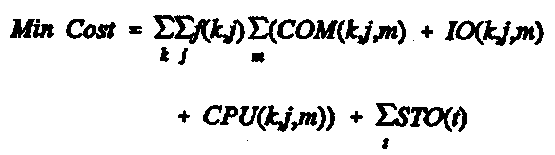
\includegraphics[scale=0.6]{CostExample-function.png}
\begin{columns}[c] % The "c" option specifies centered vertical alignment while the "t" option is used for top vertical alignment

\column{.5\textwidth} % Left column and width

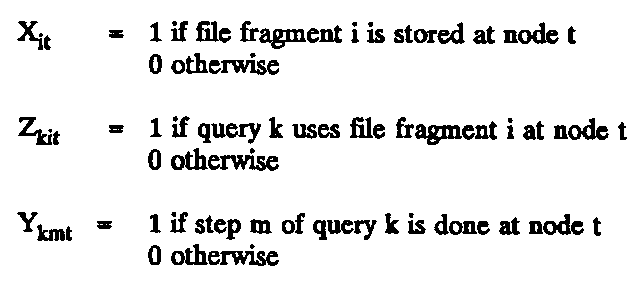
\includegraphics[scale=0.5]{CostExample-variables.png}

\column{.5\textwidth} % Right column and width
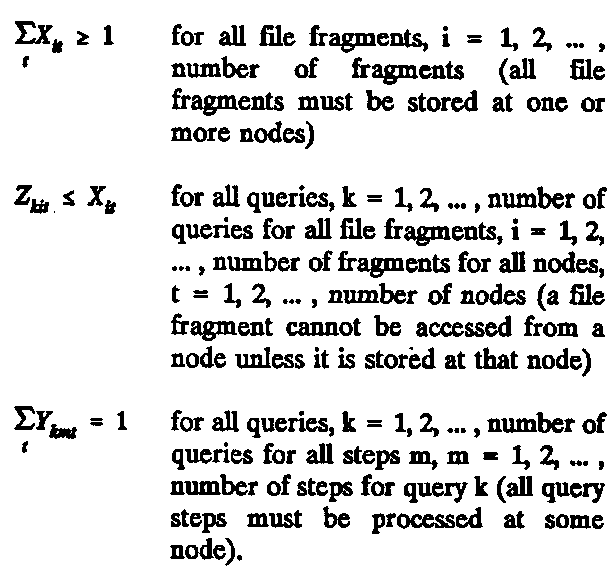
\includegraphics[scale=0.5]{CostExample-constraints.png}
\end{columns}



\end{frame}

\begin{frame}
\frametitle{Стоимостные методы (2)}
Специальные эвристические методы: методы, разработанные специально для решения подобных постановок.
\begin{itemize}
  \setlength\itemsep{1em}	
  \item Результат отказа от матметодов, одна из первых работ \cite{p13};
  \item В настоящее время~--- подход доминирует в работах с топовых конференций;
  \item В современных работах модель довольно часто убрана в оптимизатор, используются what-if вызовы;    
  \item Считается (например \cite{p10}), что они лучше чем эвристические методы общего назначения, однако \alert{...}
\end{itemize}

\end{frame}

\begin{frame}
\frametitle{Стоимостные методы (3)}

Эвристические методы общего назначения: генетические алгоритмы, алгоритмы поиска локального минимума, метод отжига, муравьиные алгоритмы, particle swarm optimization и т.п.
\begin{itemize}
  \setlength\itemsep{1em}	
  \item Модель присутствует в явном виде;
  \item Популярен в задачах размещения, хотя и не ограничен ими;
  \item Работ этого типа \alert{много}, я смотрел десятки-сотни работ.
\end{itemize}

\end{frame}

\begin{frame}
\frametitle{Смешанные методы}

Были очень популярны в 80-90-е, когда вычислительные ресурсы были ограничены.

Пример \cite{p11}, в нем:

\begin{itemize}
  \item применение процедуры, упрощение задачи;
  \item выбор финального решения с использованием стоимостной функции.
\end{itemize}
  
\center{\includegraphics[scale=0.3]{MixedExample-navathe.png}}

\end{frame}

\begin{frame}
\frametitle{Пример современной стоимостной работы (1)}

Задача \cite{p12}: выбрать атрибуты для индексирования, провести горизонтальное (хеш-фрагментирование и интервальное) и вертикальное фрагментирование для известной схемы и известного набора запросов.
\begin{itemize}
  \item Структура физического уровня~--- тройка: \\~\\ (объект, метод горизонтального \\ фрагментирования, упорядоченный набор колонок); \\~\\
  \item Объект~--- таблица + метод доступа (хип, индексы);
  \begin{itemize}
    \item Объект может быть подтаблицей.
  \end{itemize}
\end{itemize}
  
\end{frame}

\begin{frame}
\frametitle{Пример современной стоимостной работы (2)}

Конфигурация определяется как набор допустимых структур физического уровня. Допустимая структура~--- та, которую можно реализовать в данной схеме базы данных. Например, невозможно иметь два кластеризованных индекса для одной таблицы.
\\~\\
Задача~--- найти такую конфигурацию, состоящую из структур физического уровня указанных типов, которая:

\begin{enumerate}
  \setlength\itemsep{1em}	
  \item Минимизирует суммарную стоимость исполнения известного набора запросов;
  \item Укладывается в указанное ограничение на объем данных;
  \item Выполняет другие ограничения на структуры физического уровня.
\end{enumerate}

\end{frame}

\begin{frame}
\frametitle{Пример современной стоимостной работы (3)}

Постановка:

\begin{enumerate}
  \setlength\itemsep{1em}	
  \item Конфигурация системы $C$~--- набор структур физического уровня, ограничения на них, а также ограничение на объем занимаемой этими структурами памяти;
  \item Нагрузка $W$ представлена в виде набора запросов;
  \item Производительность $P$, вычисляемая как суммарное время выполнения всех запросов.
\end{enumerate}
Функция $f$, связывающая эти компоненты, представлена оптимизатором запросов в режиме what-if.

\end{frame}

\begin{frame}
\frametitle{Пример современной стоимостной работы (4)}

Этапы решения:

\begin{enumerate}
  \item Предварительный отсев вертикальных фрагментов. Цель~--- уменьшить количество вертикальных фрагментов, учитываемых в дальнейшем. Из рассмотрения исключаются те, что не несут потенциальной выгоды, и, скорее всего, не будут присутствовать в решении. Оценка выгоды производится на основании модели, учитывающей интенсивность использования атрибутов (конкретно здесь~--- frequent-itemset generation).\\~\\
  
  Используемые атрибуты берутся из запросов.
  
  \item Выбор базовых структур. Выбираются наиболее выгодные физические структуры для каждого запроса в отдельности. Для оценки применяются what-if вызовы оптимизатора;
\end{enumerate}
\end{frame}

\begin{frame}
\frametitle{Пример современной стоимостной работы (5)}

Этапы решения:

\begin{enumerate}
  \setcounter{enumi}{2}

  \item Этап слияния. Множество структур, полученных на предыдущем шаге, дополняется структурами, полученными в результате их смешивания. Этот шаг используется, например, для борьбы с чрезмерной специализацией структур;
  \item Поиск итогового решения среди структур, полученных на предыдущем шаге. Авторы работы разработали алгоритм $Greedy (m, k)$, гарантирующий оптимальный ответ при выборе $m$ структур из $k$, а для поиска остальных использующий жадный алгоритм.
\end{enumerate}
\end{frame}

\section{Горизонтальное фрагментирование}

\begin{frame}
\frametitle{Определение, свойства (1)}

\begin{block}{Горизонтальное фрагментирование}
Горизонтальное фрагментирование~--- разделение отношения на несколько отношений, каждое из которых содержит подмножество записей исходного.
\end{block}


Горизонтальное фрагментирование:
\begin{enumerate}
  \item повышает производительность СУБД за счет уменьшения объемов данных, которые потребуется обработать при выполнении запроса. Данные стремятся локализовать в одном или нескольких фрагментах меньших объемов, чем исходное отношение;
  \item свойства: полнота, восстановимость, попарное непересечение фрагментов \cite{p15};
\end{enumerate}

\end{frame}


\begin{frame}
\frametitle{Определение, свойства (2)}

\begin{block}{Горизонтальное фрагментирование}
Горизонтальное фрагментирование~--- разделение отношения на несколько отношений, каждое из которых содержит подмножество записей исходного.
\end{block}

\begin{enumerate}
  \setcounter{enumi}{2}
  \item полезно не только в распределенных, но и в централизованных СУБД;
  \item в отличии от индексов и материализованных представлений не реплицирует данные, не привносит дополнительных затрат при обновлениях и в хранении;
  \item мощный инструмент администратора базы данных, поддерживающийся практически в каждом диалекте SQL DDL.

\end{enumerate}

\end{frame}

\begin{frame}
\frametitle{Типы горизонтального фрагментирования (1): \cite{p16, p17}}

Атрибутное фрагментирование:
\small{
\begin{itemize}
  \item Интервальное фрагментирование (range data partitioning). Домены атрибутов фрагментирования делятся на несколько непересекающихся интервалов. Запись относится к фрагменту, если значение атрибута(ов) принадлежит к характеризующему интервалу.
  \item Фрагментирование с помощью хеш-функции (hash data partitioning). Принадлежность записи к конкретному фрагменту определяется хеш-функцией от атрибута(ов).
  \item Списковое фрагментирование (list partitioning)~--- каждый фрагмент задается списком допустимых значений.
  \item Виртуальное колоночное фрагментирование (virtual column partitioning). В отношение добавляется виртуальный атрибут, значение которого задается формулой от набора других. 
\end{itemize}
}
\end{frame}

\begin{frame}
\frametitle{Типы горизонтального фрагментирования (2)}

Современные СУБД поддерживают и смешанное (composite partitioning): 
\begin{itemize}
  \setlength\itemsep{1em}	
  \item range-hash: сначала интервальное, потом хеш-функция;
  \item на каждом шаге атрибуты могут различны.
\end{itemize}

Изучалось в ранних работах \cite{p41}, \cite{p38}, \cite{p40}, \cite{p39}.

\end{frame}

\begin{frame}
\frametitle{Типы горизонтального фрагментирования (3)}

Фрагментирование, не зависящее от значений атрибутов:
\begin{itemize}
  \setlength\itemsep{1em}

  \item Случайное равномерное фрагментирование (random-equal data partitioning).  Записи распределяются между фрагментами случайным образом, но так, чтобы фрагменты были равны по размеру.

  \item Круговое фрагментирование (round-robin data partitioning). Является наиболее популярной реализацией этого класса методов фрагментирования. Записи относятся к фрагментам последовательно, по кругу, в зависимости от номера.
\end{itemize}

\end{frame}

\begin{frame}
\frametitle{Типы горизонтального фрагментирования (4): сравнение}

Атрибутное фрагментирование:

\begin{itemize}
  \setlength\itemsep{1em}	
  \item Позволяет использовать сложную семантику при оптимизации запроса. Пример: интервальное позволит задействовать только один узел из набора;
  \item Склонно к асимметрии (skew) размеров фрагментов.
\end{itemize}

Фрагментирование, не зависящее от значений атрибутов:

\begin{itemize}
  \setlength\itemsep{1em}	
  \item Использование семантики невозможно;
  \item Ассиметрия отсутствует.
\end{itemize}

\end{frame}

\begin{frame}
\frametitle{Формирование фрагментов: кластеризация записей (record clustering)}

\begin{block}{}
Идея: создаем фрагменты в результате исполнения запросов, так чтобы совместно запрашиваемые данные находились в одном фрагменте. Для достижения этого предлагается, в частности, использовать различные алгоритмы кластеризации.
\end{block}

Избранные работы: \cite{p20, p19} и серия работ N. Gorla \cite{p18}.
\\~\\
Идея похожа на современное направление адаптивного индексирования (adaptive indexing) \cite{p21}.

\end{frame}

\begin{frame}
\frametitle{Формирование фрагментов: использование предикатов}

\begin{block}{}
Идея: создавать фрагменты на основании предикатов в запросах \cite{p22, p23}.
\end{block}

\begin{itemize}
  \setlength\itemsep{1em}	
  \item Очень красивая и влиятельная идея, породила массу работ--последователей, включая смежные области~--- вертикальное фрагментирование \cite{p24}, фрагментирование хранилищ данных \cite{p25}, фрагментирование в объектных СУБД \cite{p26}.

  \item Метод получения фрагментов (хорошо описан в \cite{p15}) напоминает алгоритм Ханта (Hunts algorithm)~--- алгоритм для построения дерева решений.

  \item О применении на практике мне ничего не известно.

\end{itemize}

\end{frame}

\begin{frame}
\frametitle{Формирование фрагментов: распространение по ключам}

\begin{block}{}
Работа \cite{p23} делит методы фрагментирования на основные (primary partitioning)  и производные (derived).
\end{block}

\begin{block}{}
Основное фрагментирование отношения определяется только значениями собственных атрибутов, в то время как производное дополнительно зависит и от фрагментов другого отношения. 
\end{block}

\begin{block}{}
Производное фрагментирование применяется при фрагментировании отношения, связанного посредством внешнего ключа с некоторым другим. Идея: сформировать фрагменты таким образом, чтобы каждому фрагменту первого отношения сопоставлялся фрагмент второго. 
\end{block}

\end{frame}

\begin{frame}
\frametitle{Формирование фрагментов: распространение по ключам}

\begin{enumerate}
  \setlength\itemsep{1em}	
  \item Этот метод позволяют получать цепочки фрагментирования наборов отношений, связанных ключами;
  \item В современных работах \cite{p16} эти два типа фрагментирования называются моно фрагментирование (mono) и таблице-зависимое (table-dependent);
  \item Ранняя реализация на практике \cite{p42}, интересный факт~--- цепочек длины больше чем 3 не бывает;
  \item В СУБД Oracle 11gR1 сделали поддержку в 2008 году \cite{p27}, называют ссылочное (referential).
\end{enumerate}

\end{frame}

\section{Размещение данных}

\begin{frame}
\frametitle{Размещение данных (1)}

Задача горизонтального фрагментирования часто рассматривается в условиях распределенной СУБД, тогда она решается совместно с задачей размещения данных.
\\~\\
Цели размещения данных:
\begin{itemize}
  \setlength\itemsep{1em}	
  \item Повышение производительности;
  \item Повышение надежности;
  \item Балансировка нагрузки.
\end{itemize}

Как самостоятельная задача это наиболее старая из всех задач о выборе структур физического уровня, происходит от задачи о размещении файла в компьютерной сети.

\end{frame}


\begin{frame}
\frametitle{Размещение данных (2): типы}

Типы \cite{p28}:
\begin{enumerate}
  \setlength\itemsep{1em}	
  \item Чистое размещение данных (data allocation)~--- размещение только фрагментов данных, с целью увеличения производительности или повышения надежности системы. Подавляющее большинство рассмотренных работ относятся к этому классу.
  \item Размещение данных и запросов (data and query allocation)~--- постановка размещает еще и запросы. 
  \item Размещение пользовательской нагрузки (user load allocation)~--- постановка размещает только запросы.
\end{enumerate}

\end{frame}

\begin{frame}
\frametitle{Типы постановок задачи размещения данных}

Задача размещения бывает поставлена в двух вариантах \cite{p32}:

\begin{itemize}
  \setlength\itemsep{1em}	
  \item Неизбыточное размещение, при котором каждый фрагмент или отношение находится ровно на одном узле;
  \item Избыточное размещение, то есть репликация, может применяться для повышения надежности или производительности СУБД.
\end{itemize}

\end{frame}


\begin{frame}
\frametitle{Размещение данных (3): постановка задачи}

Постановка задачи размещения данных описывается схемой, однако требуются некоторые уточнения:

\begin{enumerate}
  \setlength\itemsep{1em}	
  \item Аппаратная конфигурация включает в себя число узлов и их характеристики. Также описываются параметры сети.
  \item Искомая конфигурация физического уровня должна сопоставлять каждому фрагменту узел и при этом не нарушать ограничения (например, объем жесткого диска узла не должен быть превышен).
  \item В качестве метрики $P$ дополнительно может выступать суммарный объем переданных по сети данных. Бывают и многокомпонентные метрики, но всё-равно, передача по сети вносит значительный вклад. 
\end{enumerate}

\end{frame}

\begin{frame}

\frametitle{Размещение данных и фрагментирование}

\begin{block}{}
Один из острейших вопросов данной области исследований~--- целесообразно ли разрабатывать метод распределения данных в отрыве от фрагментирования (итеративный дизайн \cite{p29, p30}) или же следует решать эти два аспекта совместно (комбинированный или интегрированный \cite{p31} дизайн). 
\end{block}

\begin{itemize}
  \setlength\itemsep{1em}	
  \item Комбинированный недостаточно гибок и очень трудоемок.
  \item Итеративное решение хуже, теряется часть семантики.
\end{itemize}

В итоге, данная проблема привела к появлению двух независимых сообществ исследователей \cite{p29}.

\end{frame}

\begin{frame}

\frametitle{Принцип локальности ссылки}

\begin{block}{}

Движущий принцип как размещения, так и фрагментирования~--- ``локальность ссылки'' (locality of reference) \cite{p8}.
\\~\\
Идея: делаем совместное хранение данных для данных, которые будут совместно запрашиваться. Причем, идея применяется ко всему: будь то записи внутри фрагмента, фрагменты внутри узла и пр. Во многих случаях это позволяет снизить стоимость обработки запроса. Согласно \cite{p32} в хорошо спроектированной базе данных, 90\% обращений к данным должны быть локальными. 
\end{block}

Значительное количество работ опирается на данную идею.

\end{frame}

\begin{frame}
\frametitle{Исторический экскурс}

Задача о размещении данных в контексте СУБД ``выросла'' из задачи о размещении файла в компьютерных сетях. Самая первая найденная мной работа \cite{p2}.

Почему выросла:
\begin{itemize}
  \item Заимствованные подходы оказались слабо приспособленными: модели не учитывали специфику исполнения запросов в СУБД (например, необходимость узлов обмениваться информацией друг с другом при выполнении реляционной операции соединения).
\end{itemize}
  
Обзор работ данной тематики, представлено более десяти типов моделей для задачи о размещении файлов \cite{p33}. Классифицируют по метрике, количеству копий и методу решения.
\end{frame}

\begin{frame}
\frametitle{Модели для размещения данных в контексте СУБД}

Классификация моделей для размещения данных в контексте СУБД:
\begin{enumerate}
  \setlength\itemsep{1em}		
  \item Модели, учитывающие проведение распределенных транзакций. В качестве параметров в них дополнительно может фигурировать стоимость запроса замка или количество сообщений, которые необходимо передать;
  \item Модели, требующие обеспечения определенного уровня надежности;
  \item Модели, учитывающие характер и стоимости отдельных реляционных операторов (например, оператора соединения), составляющих план запроса.
\end{enumerate}

Ссылок очень много, есть в статье.

\end{frame}

\begin{frame}
\frametitle{Динамическая постановка задачи и миграция данных}

\begin{block}{}
Первые работы по размещению данных рассматривали задачу в статическом контексте~--- когда ни запросы, ни данные не изменяются. 
\\~\\
Однако со временем нагрузка может меняться или уточняться, может поменяться топология сети \cite{p34} и т.д. Это может негативно сказаться на производительности системы.

\end{block}{}

Поэтому позже появились работы, изучавшие и миграцию (migration) данных \cite{p34}, \cite{p35}, \cite{p36}, \cite{p37} в условиях меняющейся нагрузки. 

\end{frame}

\begin{frame}
\frametitle{Общая схема решения задачи в динамической постановке}

В результате миграции данных обеспечивается выравнивание загрузки узлов при исполнении запросов. То есть, можно сказать, что в данных работах решается задача балансировки нагрузки.

\begin{enumerate}
  \setlength\itemsep{1em}		
  \item Собирается статистика обращения к фрагментам (например, с помощью счетчиков);

  \item Через определенный промежуток времени или по выполнению определенных условий (например, появлению новых запросов) производится анализ существующей конфигурации;

  \item В зависимости от пороговых значений счетчиков или потенциальной стоимости новой конфигурации принимается решение об изменениях~--- миграции фрагмента на другой узел или его изменении (расщеплении или слиянии с другим). 
\end{enumerate}
\end{frame}

\begin{comment}

\begin{frame}
\frametitle{Полная и частичная декластеризация (1)}

\begin{block}{}

Полной декластеризацией (full declustering) \cite{p43} называется специальный метод горизонтального фрагментирования и размещения отношения. 
\\~\\
Идея: сначала отношение горизонтально фрагментируется на количество частей, равное числу узлов в системе, а затем, они размещаются так, чтобы на одном узле находился один фрагмент. Частичная декластеризация (partial declustering)~--- аналогична, но рассматривается строгое подмножество всех узлов системы.
\\~\\
Взаимно-однозначное соответствие элементов множества фрагментов и элементов множества всех узлов системы.
\end{block}{}

\end{frame}

\begin{frame}
\frametitle{Полная и частичная декластеризация (2)}

\begin{itemize}
  \item Экспериментальные сравнения методов \cite{p44, p43, p46, p41}.
  \item В \cite{p46} изучалось влияние четырех стратегий балансировки нагрузки в случае частичной или полной декластеризации. 
  \item Декластеризация набора отношений и метод выбора ключа декластеризации рассматривается в \cite{p44, p45}. 
\end{itemize}

\end{frame}


\begin{frame}
\frametitle{Современные работы по фрагментированию и размещению (1): what-if}

Большинство современных работ используют what-if подход \cite{p47}:

\begin{itemize}
 
  \item метод оценки конфигурации без затрат на ее создание и выполнение над ней запросов. 
  \item привлекательность конфигурации оценивается исходя из статистической информации и метаданных. 
  \item функция впервые появилась \cite{p48} в работе \cite{p49}, а ныне она встроена в практически все современные СУБД. 

\end{itemize}
\end{frame}

\begin{frame}
\frametitle{Современные работы по фрагментированию и размещению (2): общая схема}

Можно утверждать, что большинство современных работ следуют единому процессу решения задачи о выборе структур физического уровня \cite{p47}.
\begin{enumerate}
  \item Поиск структур-кандидатов. На этом этапе из набора запросов выделяются потенциально выгодные структуры путем осуществления отбора с потерями;
  \item Различные процедуры расширения списка кандидатов, такие как комбинирование различных составляющих этих структур;
  \item Некоторая процедура отбора. Это, зачастую, итеративный процесс, конструирующий решение снизу вверх путем добавления одной структуры на каждом шаге и использующий what-if метод. 
\end{enumerate}

\end{frame}


\begin{frame}
\frametitle{Коммерческие СУБД и современные работы по фрагментированию и размещению: DB2 \cite{p50}}

Исследование \cite{p50} решает задачу фрагментирования отношений в условиях распределенной СУБД без совместного использования ресурсов  (shared-nothing). Кроме фрагментов, дополнительно учитывались и материализованные представления. Для решения этой задачи авторы предлагают интегрировать модуль поиска фрагментов и оптимизатор запросов. Предыдущие работы \cite{p50}:

\begin{enumerate}
  \item Не встраивали поиск альтернатив внутрь оптимизатора;
  \item Часто использовали свои стоимостные модели, не связанные с моделями оптимизатора, что может привести к выбору неоптимального решения и, как следствие, худшей производительности.
\end{enumerate}

\end{frame}

\begin{frame}
\frametitle{Коммерческие СУБД и современные работы по фрагментированию и размещению: DB2 \cite{p50}}

Расширили функционал оптимизатора двумя режимами:
\begin{enumerate}
  \item ``рекомендация'', оптимизатор накапливает потенциальные решения задачи фрагментирования для каждого запроса в отдельности. Затем, для каждого из них находит оптимальный план и варианты фрагментирования. 
  \item ``вычисление'' оптимизатор подставляет найденную на предыдущем шаге конфигурацию и использует ее при оптимизации запросов. Заметим, что результатом работы в этих двух режимах является сгенерированная структура (план выполнения запроса), никакие дополнительные дорогостоящие действия не предпринимаются, выполнения запроса не происходит. 
\end{enumerate}

Достоверные эксперименты на TPC-H, превзошли генетический.

\end{frame}

\begin{frame}
\frametitle{Коммерческие СУБД и современные работы по фрагментированию и размещению: DB2 \cite{p51}}

Продолжение предыдущей работы \cite{p50}, рассматривается вопрос построения системы, которая бы учитывала несколько различных типов физических структур.
\\~\\
Кроме фрагментирования предлагается учитывать индексы, материализованные представления и структуры многомерной кластеризации. В деталях про каждый отдельный компонент рассказывается в \cite{p50, p52, p53}.
\end{frame}


\begin{frame}
\frametitle{Коммерческие СУБД и современные работы по фрагментированию и размещению: DB2 \cite{p51}}

Обсуждается вопрос о выборе подхода к реализации многокомпонентных рекомендательных систем:
\begin{itemize}
  \item Итеративный подход ~--- решает задачу нахождения структур каждого типа последовательно, для каждой компоненты в отдельности. Отдельные алгоритмы рассматриваются как ``черный ящик'';
  \item Интегрированный подход: ищется решение для компонентов всех типов одновременно одним алгоритмом;
  \item \alert{Гибридный подход: оценивание степени влияния компонент одного типа на другой для выявления  зависимостей и благоприятного порядка обработки. Предложенный алгоритм по природе итеративен, однако выбирать все компоненты он может несколько раз, в цикле.}
\end{itemize}
\end{frame}

\begin{frame}
\frametitle{Коммерческие СУБД и современные работы по фрагментированию и размещению: Microsoft SQL Server 2008 Parallel Data Warehouse \cite{p54}}

Работа \cite{p54}: фрагментирование, размещение с репликацией.
\\~\\
Идея глубокой интеграции рекомендательной подсистемы с оптимизатором. Критика использования what-if методов в современном виде:

\begin{enumerate}
  \item Слабая масштабируемость данного подхода. При увеличении числа таблиц, число возможных конфигураций растет экспоненциально и увеличивает количество необходимых вызовов оптимизатора;
  \item Узость API между тюнером и оптимизатором СУБД;
\end{enumerate}
\end{frame}

\begin{frame}
\frametitle{Коммерческие СУБД и современные работы по фрагментированию и размещению: Microsoft SQL Server 2008 Parallel Data Warehouse \cite{p54}}

\begin{enumerate}
  \setcounter{enumi}{2}
  \item Неэффективность. Каждый вызов оптимизатора тратит много ресурсов на подготовку к работе. Дополнительные затраты~--- синтаксический анализ запроса, проверка корректности, проверка ограничений безопасности и другая сопутствующая деятельность, не связанная с фрагментированием. В итоге, на работу с конфигурациями будет тратиться лишь малая доля общего времени.  
\end{enumerate}

\begin{block}{}
Для решения этих проблем авторы предлагают встраивание компонента рекомендации фрагментов в оптимизатор и параллелизацию поиска оптимальной конфигурации. 
\end{block}{}

\end{frame}


\begin{frame}
\frametitle{Коммерческие СУБД и современные работы по фрагментированию и размещению: Microsoft SQL Server \cite{p55}}

Очень много качественных работ по выбору индексов \cite{p55}, однако рассматривать не будем ввиду ограниченности времени и несоответствия тематики.

\end{frame}

\begin{frame}
\frametitle{Коммерческие СУБД и современные работы по фрагментированию и размещению: PostgreSQL}

Средство выбора индексов и фрагментов для СУБД PostgreSQL представлено в \cite{p56, p57}. Компонента рекомендации фрагментов взят из средства AutoPart \cite{p58}. 

\end{frame}
\end{comment}


\begin{frame}[fragile]
\frametitle{Коммерческие СУБД и современные работы по фрагментированию и размещению}

\begin{itemize}
    \setlength\itemsep{1em}		
	\item DB2: индексы, материализованные представления, и структуры многомерной кластеризации \cite{p51}
	\item Microsoft SQL Server: индексы (семейство работ), вертикальное фрагментирование \cite{p55}
	\item Microsoft SQL Server 2008 Parallel Data Warehouse: фрагментирование, размещение с репликацией \cite{p54}
	\item PostgreSQL: фрагменты, индексы \cite{p56, p57, p58}
	\item ...
\end{itemize}

\end{frame}


\begin{comment}
\begin{frame}
\frametitle{Перспективные направления}

\small

\begin{enumerate}
  \item Глубокая интеграция с оптимизатором~--- параллелизм, кеширование планов и т.д. \cite{p47, p60, p10};
  \item Он-лайн тюниг \cite{p61, p62, p56};
  \item Новые методы фрагментирования, новые физические структуры и т.д. \cite{p64, p63, p27};
  \item Виртуальное фрагментирование \cite{p59};
  \item Более точные модели, специальные модели точно описывающие предметную область \cite{p58, p65};
  \item Оценка качества тюнеров, сравнение \cite{p67, p66, p69, p68};
  \item Построение многокомпонентых тюнеров \cite{p51}.
\end{enumerate}

\end{frame}
\end{comment}

\begin{frame}
\frametitle{Статья}

Ввиду ограниченности времени смотрите в старой статье:

\begin{block}{}
	Г. А. Чернышев, ``Обзор подходов к организации физического уровня в СУБД'', Тр. СПИИРАН, 24 (2013), 222--276. url: \url{http://www.mathnet.ru/php/archive.phtml?wshow=paper&jrnid=trspy&paperid=580&option_lang=rus}
\end{block}{}

\end{frame}


\begin{comment}

\begin{frame}
\frametitle{Спасибо!}
\begin{block}{}
К сожалению, даже рассказывая на уровне определений и классификаций удалось уместить только половину того, что я хотел. За бортом остались: 
\begin{enumerate}
  \item вертикальное фрагментирование; 
  \item фрагментирование для хранилищ данных; 
  \item небольшой кусочек про материализованные представления;
  \item список проблем области в целом.
\end{enumerate}

\end{block}{}
    
\end{frame}
\end{comment}

%------------------------------------------------
\begin{frame}[allowframebreaks]
\frametitle{Ссылки}
\footnotesize{
\begin{thebibliography}{99} % Beamer does not support BibTeX so references must be inserted manually as below
%\bibitem[Smith, 2012]{p1} John Smith (2012)
%\newblock Title of the publication
%\newblock \emph{Journal Name} 12(3), 45 -- 678.
%\newblock 

\bibitem[Hoffer, 1975] {p1} Hoffer J. A., Severance D. G. The use of cluster analysis in physical data base design // Proceedings of the 1st International Conference on Very
Large Data Bases. VLDB ’75. New York, NY, USA : ACM, 1975. P. 69--86.
URL: http://doi.acm.org/10.1145/1282480.1282486.

\bibitem[Chu, 1969] {p2} Chu W. W.  Optimal file allocation in a multiple computer system // IEEE Trans. Comput. 1969. Vol. 18, no. 10. P. 885--889. URL: http://dx.doi.org/10.1109/T-C.1969.222542.

\bibitem[Lightstone, 2009] {p3} Lightstone S. Physical database design for relational databases // Encyclopedia of Database Systems / Ed. by Ling Liu, M.Tamer \''{O}ZSU. Springer US, 2009. P. 2108--2114. URL: http://dx.doi.org/10.1007/978-0-387-39940-9\_644.

\bibitem[Chaudhuri, 2009] {p4} Chaudhuri S., Weikum G. Self-management technology in databases // Encyclopedia of Database Systems / Ed. by Ling Liu, M.Tamer \''{O}zsu.
Springer US, 2009. P. 2550--2555. URL: http://dx.doi.org/10.1007/978-0-387-39940-9\_334.

\bibitem[Agrawal, 2006] {p5} Agrawal S., Chu E., Narasayya V. Automatic physical design tuning: workload as a sequence // Proceedings of the 2006 ACM SIGMOD international conference on Management of data. SIGMOD ’06. New York, NY, USA : ACM, 2006. P. 683--694. URL: http://doi.acm.org/10.1145/1142473.1142549

\bibitem[Agrawal, 2004] {p6} Database tuning advisor for Microsoft SQL Server 2005 / Sanjay Agrawal, Surajit Chaudhuri, Lubor Kollar et al. // Proceedings of VLDB. 2004. P. 1110--1121.

\bibitem[Navathe, 1989] {p7} Navathe S. B., Ra M. Vertical partitioning for database design: a graphical algorithm // Proceedings of the 1989 ACM SIGMOD international conference on Management of data. SIGMOD ’89. New York, NY, USA : ACM, 1989. P. 440--450. URL: http://doi.acm.org/10.1145/67544.66966.

\bibitem[Tamhankar, 1998] {p8} Tamhankar A. M., Ram S. Database fragmentation and allocation: an integrated methodology and case study // Trans. Sys. Man Cyber. Part A. 1998. Vol. 28, no. 3. P. 288--305. URL: http://dx.doi.org/10.1109/3468.668961.

\bibitem[March, 1995] {p9} March S. T., Rho S. Allocating data and operations to nodes in distributed database design // IEEE Trans. on Knowl. and Data Eng. 1995. Vol. 7, no. 2. P. 305--317. URL: http://dx.doi.org/10.1109/69.382299.

\bibitem[Nehme, 2011] {p10} Nehme R., Bruno N. Automated partitioning design in parallel database systems // Proceedings of the 2011 international conference on Management of data. SIGMOD ’11. New York, NY, USA : ACM, 2011. P. 1137--1148. URL: http://doi.acm.org/10.1145/1989323.1989444.

\bibitem[Navathe, 1984] {p11} Vertical partitioning algorithms for database design / Shamkant Navathe, Stefano Ceri, Gio Wiederhold, Jinglie Dou // ACM Trans. Database Syst. 1984. Vol. 9. P. 680--710. URL: http://doi.acm.org/10.1145/1994.2209.

\bibitem[Agrawal, 2004] {p12} Agrawal S., Narasayya V., Yang B. Integrating vertical and horizontal partitioning into automated physical database design // Proceedings of the 2004 ACM SIGMOD international conference on Management of data. SIGMOD ’04. New York, NY, USA : ACM, 2004. P. 359--370. URL: http://doi.acm.org/10.1145/1007568.1007609.

\bibitem[Hammer, 1979] {p13} Hammer M., Niamir B. A heuristic approach to attribute partitioning // Proceedings of the 1979 ACM SIGMOD international conference on Management of data. SIGMOD ’79. New York, NY, USA : ACM, 1979. P. 93--101. URL: http://doi.acm.org/10.1145/582095.582110.

\bibitem[Papadomanolakis, 2007] {p14} Papadomanolakis S., Ailamaki A. An integer linear programming approach to database design // Proceedings of the 2007 IEEE 23rd International Conference on Data Engineering Workshop. ICDEW ’07. Washington, DC, USA : IEEE Computer Society, 2007. P. 442--449. URL: http://dx.doi.org/10.1109/ICDEW.2007.4401027

\bibitem[\"{O}zsu, 1999] {p15} {\"O}zsu M. T., Valduriez P. Principles of distributed database systems (2nd ed.). Upper Saddle River, NJ, USA : Prentice-Hall, Inc., 1999. ISBN: 0-13-659707-6.

\bibitem[Bellatreche, 2009] {p16} Bellatreche L., Woameno K. Y. Dimension table driven approach to referential partition relational data warehouses // Proceedings of the ACM twelfth international workshop on Data warehousing and OLAP. DOLAP ’09. New York, NY, USA : ACM, 2009. P. 9--16. URL: http://doi.acm.org/10.1145/1651291.1651294.

\bibitem[Taniar, 2008] {p17} High Performance Parallel Database Processing and Grid Databases / David Taniar, Clement H. C. Leung, Wenny Rahayu, Sushant Goel. Wiley Publishing, 2008. ISBN: 0470107626, 9780470107621.

\bibitem[Gorla, 2003] {p18} Applying genetic algorithms in database partitioning / Vincent Ng, Dik Man Law, Narasimhaiah Gorla, Chi Kong Chan // Proceedings of the 2003 ACM symposium on Applied computing. SAC ’03. New York, NY, USA : ACM, 2003. P. 544--549. URL: http://doi.acm.org/10.1145/952532.952639.

\bibitem[Moghrabi, 2000] {p19} Moghrabi I., Makholian R. A new approach to clustering records in information retrieval systems // Information Retrieval. 2000. Vol. 3. P. 105--126. 10.1023/A:1009901830009. URL: http://dx.doi.org/10.1023/A:1009901830009.

\bibitem[Bell, 1984] {p20} Bell D. A. Physical record clustering in databases // Kybernetes. 1984. Vol. 13. P. 31--37.

\bibitem[Idreos, 2007] {p21} Idreos S., Kersten M. L., Manegold S. Database cracking // CIDR. www.cidrdb.org, 2007. P. 68--78.

\bibitem[Ceri, 1982] {p22} Ceri S., Negri M., Pelagatti G. Horizontal data partitioning in database design // Proceedings of the 1982 ACM SIGMOD international conference on Management of data. SIGMOD ’82. New York, NY, USA : ACM, 1982. P. 128--136. URL: http://doi.acm.org/10.1145/582353.582376.

\bibitem[Ceri, 1983] {p23} Ceri S., Navathe S., Wiederhold G. Distribution design of logical database schemas // IEEE Transactions on Software Engineering. 1983. Vol. 9. P. 487--504.

\bibitem[Zhang, 1994] {p24} Zhang Y., Orlowska M. E. On fragmentation approaches for distributed database design // Information Sciences - Applications. 1994. Vol. 1, no. 3. P. 117--132. URL: http://www.sciencedirect.com/science/article/pii/1069011594900051.

\bibitem[Noaman, 1999] {p25} Noaman A. Y., Barker K. A horizontal fragmentation algorithm for the fact relation in a distributed data warehouse // Proceedings of the eighth international conference on Information and knowledge management. CIKM ’99. New York, NY, USA : ACM, 1999. P. 154--161. URL: http://doi.acm.org/10.1145/319950.319972.

\bibitem[Bellatreche, 2000] {p26} Bellatreche L., Karlapalem K., Simonet A. Algorithms and support for horizontal class partitioning in object-oriented databases // Distributed and Parallel Databases. 2000. Vol. 8. P. 155--179. 10.1023/A:1008745624048. URL: http://dx.doi.org/10.1023/A:1008745624048.

\bibitem[Eadon, 2008] {p27} Supporting table partitioning by reference in oracle / George Eadon, Eugene Inseok Chong, Shrikanth Shankar et al. // Proceedings of the 2008 ACM SIGMOD international conference on Management of data. SIGMOD ’08. New York, NY, USA : ACM, 2008. P. 1111--1122. URL: http://doi.acm.org/10.1145/1376616.1376727.

\bibitem[Oates, 2001] {p28} Oates M. J., Corne D. W. Global web server load balancing using evolutionary computational techniques // Soft Computing. 2001. Vol. 5, no. 4. P. 297--312. URL: http://dx.doi.org/10.1007/s005000100103

\bibitem[Bellatreche, 2009] {p29} Bellatreche L., Benkrid S. A joint design approach of partitioning and allocation in parallel data warehouses // Data Warehousing and Knowledge Discovery / Ed. by Torben Pedersen, Mukesh Mohania, A Tjoa. Springer Berlin / Heidelberg, 2009. Vol. 5691 of Lecture Notes in Computer Science. P. 99--110. 10.1007/978-3-642-03730-6 9. URL: http://dx.doi.org/10.1007/978-3-642-03730-6\_9.

\bibitem[Bellatreche, 2010] {p30} Bellatreche L., Cuzzocrea A., Benkrid S. F\&{A}: a methodology for effectively and efficiently designing parallel relational data warehouses on heterogenous database clusters // Proceedings of the 12th international conference on Data warehousing and knowledge discovery. DaWaK’10. Berlin, Heidelberg : Springer-Verlag, 2010. P. 89--104. URL: http://dl.acm.org/citation.cfm?id=1881923.1881934.

\bibitem[Zilio, 2004] {p31} DB2 design advisor: integrated automatic physical database design / Daniel C. Zilio, Jun Rao, Sam Lightstone et al. // Proceedings of the Thirtieth international conference on Very large data bases - Volume 30. VLDB ’04. VLDB Endowment, 2004. P. 1087--1097. URL: http://dl.acm.org/citation.cfm?id=1316689.1316783.

\bibitem[Ceri, 1987] {p32} Ceri S., Pernici B., Wiederhold G. Distributed database design methodologies // Proceedings of the IEEE. 1987. Vol. 75, no. 5. P. 533--546.

\bibitem[Dowdy, 1982] {p33} Dowdy L. W., Foster D. V. Comparative models of the file assignment problem // ACM Comput. Surv. 1982. Vol. 14, no. 2. P. 287–313. URL: http://doi.acm.org/10.1145/356876.356883.

\bibitem[Rivera-Vega, 1990] {p34} Rivera-Vega P., Varadarajan R., Navathe S. Scheduling data redistribution in distributed databases // Data Engineering, 1990. Proceedings. Sixth International Conference on. 1990. feb. P. 166--173.

\bibitem[Brunstrom, 1995] {p35} Brunstrom A., Leutenegger S. T., Simha R. Experimental evaluation of dynamic data allocation strategies in a distributed database with changing workloads // Proceedings of the fourth international conference on Information and knowledge management. CIKM ’95. New York, NY, USA : ACM, 1995. P. 395--402. URL: http://doi.acm.org/10.1145/221270.221652.

\bibitem[Hauglid, 2010] {p36} Hauglid J. O., Ryeng N. H., N{\o}rv{\aa}g K. Dyfram: dynamic fragmentation and replica management in distributed database systems // Distrib. Parallel Databases. 2010. Vol. 28. P. 157--185. URL: http://dx.doi.org/10.1007/s10619-010-7068-1.

\bibitem[Kamali, 2011] {p37} Kamali S., Ghodsnia P., Daudjee K. Dynamic data allocation with replication in distributed systems // Performance Computing and Communications Conference (IPCCC), 2011 IEEE 30th International. 2011. nov. P. 1--8.

\bibitem[Ghandeharizadeh, 1990] {p38} Ghandeharizadeh S., DeWitt D. J. Hybrid-range partitioning strategy: A new declustering strategy for multiprocessor database machines // Proceedings of the 16th International Conference on Very Large Data Bases. VLDB ’90. San Francisco, CA, USA : Morgan Kaufmann Publishers Inc., 1990. P. 481--492. URL: http://dl.acm.org/citation.cfm?id=645916.671988.

\bibitem[Ghandeharizadeh, 1994] {p39} Ghandeharizadeh S., DeWitt D. J. Magic: A multiattribute declustering mechanism for multiprocessor database machines // IEEE Trans. Parallel Distrib. Syst. 1994. Vol. 5, no. 5. P. 509--524. URL: http://dx.doi.org/10.1109/71.282561.

\bibitem[Ghandeharizadeh, 1992] {p40} Ghandeharizadeh S., DeWitt D. J., Qureshi W. A performance analysis of alternative multi-attribute declustering strategies // SIGMOD Rec. 1992. Vol. 21, no. 2. P. 29--38. URL: http://doi.acm.org/10.1145/141484.130293.

\bibitem[Copeland, 1988] {p41} Data placement in Bubba / George Copeland, William Alexander, Ellen Boughter, Tom Keller // Proceedings of the 1988 ACM SIGMOD international conference on Management of data. SIGMOD ’88. New York, NY, USA : ACM, 1988. P. 99--108. URL: http://doi.acm.org/10.1145/50202.50213.

\bibitem[Didriksen, 1995] {p42} Didriksen T., Galindo-Legaria C. A., Dahle E. Database de-centralization --- a practical approach // Proceedings of the 21th International Conference on Very Large Data Bases. VLDB ’95. San Francisco, CA, USA : Morgan Kaufmann Publishers Inc., 1995. P. 654--665. URL: http://dl.acm.org/citation.cfm?id=645921.673313.

\bibitem[Mehta, 1997] {p43} Mehta M., DeWitt D. J. Data placement in shared-nothing parallel database systems // The VLDB Journal. 1997. Vol. 6. P. 53--72. URL: http://dx.doi.org/10.1007/s007780050033.

\bibitem[Zilio, 1994] {p44} Partitioning key selection for a shared-nothing parallel database system : Rep. : IBM Research Report RC 19820 (87739) / IBM T.J. Watson Research Center ; Executor: Daniel C. Zilio, Anant Jhingran, Sriram Padmanabhan : 1994.

\bibitem[Zilio, 1998] {p45} Zilio D. C. Physical database design decision algorithms and concurrent reorganization for parallel database systems : Ph. D. thesis / Daniel Costante Zilio ; University of Toronto. Toronto, Ont., Canada, Canada, 1998. AAINQ35386.

\bibitem[Rahm, 1998] {p46} Rahm E., Marek R. Analysis of dynamic load balancing strategies for parallel shared nothing database systems // Proceedings of the 19th International Conference on Very Large Data Bases. VLDB ’93. San Francisco, CA, USA : Morgan Kaufmann Publishers Inc., 1993. P. 182--193. URL: http: //portal.acm.org/citation.cfm?id=645919.672662.

\bibitem[Bruno, 2005] {p47} Bruno N., Chaudhuri S. Automatic physical database tuning: a relaxation-based approach // Proceedings of the 2005 ACM SIGMOD international conference on Management of data. SIGMOD ’05. New York, NY, USA : ACM, 2005. P. 227--238. URL: http://doi.acm.org/10.1145/1066157.1066184.

\bibitem[Maier, 2010] {p48} PARINDA: an interactive physical designer for PostgreSQL / Cristina Maier, Debabrata Dash, Ioannis Alagiannis et al. // Proceedings of the 13th International Conference on Extending Database Technology. EDBT ’10. New York, NY, USA : ACM, 2010. P. 701--704. URL: http://doi.acm.org/10.1145/1739041.1739131.

\bibitem[Finkelstein, 1988] {p49} Finkelstein S., Schkolnick M., Tiberio P. Physical database design for relational databases // ACM Trans. Database Syst. 1988. Vol. 13. P. 91--128. URL: http://doi.acm.org/10.1145/42201.42205.

\bibitem[Rao, 2002] {p50} Automating physical database design in a parallel database / Jun Rao, Chun Zhang, Nimrod Megiddo, Guy Lohman // Proceedings of the 2002 ACM SIGMOD international conference on Management of data. SIGMOD ’02. New York, NY, USA : ACM, 2002. P. 558–569. URL: http://doi.acm.org/10.1145/564691.564757.

\bibitem[Zilio, 2004a] {p51} {DB2} design advisor: integrated automatic physical database design / Daniel C. Zilio, Jun Rao, Sam Lightstone et al. // Proceedings of the Thirtieth international conference on Very large data bases - Volume 30. VLDB ’04. VLDB Endowment, 2004. P. 1087--1097. URL: http://dl.acm.org/citation.cfm?id=1316689.1316783.

\bibitem[Lightstone, 2004a] {p52} Lightstone S. S., Bhattacharjee B. Automated design of multidimensional clustering tables for relational databases // Proceedings of the Thirtieth international conference on Very large data bases - Volume 30. VLDB ’04. VLDB Endowment, 2004. P. 1170--1181. URL: http://dl.acm.org/citation.cfm?id=1316689.1316789.

\bibitem[Zilio, 2004b] {p53} Recommending materialized views and indexes with the {IBM DB2} design advisor / D.C. Zilio, C. Zuzarte, S. Lightstone et al. // Autonomic Computing, 2004. Proceedings. International Conference on. 2004. may. P. 180--187.

\bibitem[Nehme, 2011] {p54} Nehme R., Bruno N. Automated partitioning design in parallel database systems // Proceedings of the 2011 international conference on Management of data. SIGMOD ’11. New York, NY, USA : ACM, 2011. P. 1137--1148. URL: http://doi.acm.org/10.1145/1989323.1989444.

\bibitem[Chaudhuri, 2007] {p55} Chaudhuri S., Narasayya V. Self-tuning database systems: a decade of progress // Proceedings of the 33rd international conference on Very large
data bases. VLDB ’07. VLDB Endowment, 2007. P. 3--14. URL: http://dl.acm.org/citation.cfm?id=1325851.1325856.

\bibitem[Alagiannis, 2010] {p56} An automated, yet interactive and portable DB designer / Ioannis Alagiannis, Debabrata Dash, Karl Schnaitter et al. // Proceedings of the 2010 ACM SIGMOD International Conference on Management of data. SIGMOD ’10. New York, NY, USA : ACM, 2010. P. 1183--1186. URL: http://doi.acm.org/10.1145/1807167.1807314.

\bibitem[Maier, 2010] {p57} PARINDA: an interactive physical designer for PostgreSQL / Cristina Maier, Debabrata Dash, Ioannis Alagiannis et al. // Proceedings of the 13th International Conference on Extending Database Technology. EDBT ’10. New York, NY, USA : ACM, 2010. P. 701--704. URL: http://doi.acm.org/10.1145/1739041.1739131.

\bibitem[Papadomanolakis, 2004] {p58} Papadomanolakis S., Ailamaki A. AutoPart: automating schema design for large scientific databases using data partitioning // Scientific and Statistical Database Management, 2004. Proceedings. 16th International Conference on. 2004. june. P. 383--392.

\bibitem[Lima, 2009] {p59} Parallel OLAP query processing in database clusters with data replication / Alexandre Lima, A., Camille Furtado, Patrick Valduriez, Marta Mattoso // Distributed and Parallel Databases. 2009. Vol. 25, no. 1-2. P. 97--123. URL: http://hal.inria.fr/inria-00482183.

\bibitem[Papadomanolakis, 2007] {p60} Papadomanolakis S., Dash D., Ailamaki A. Efficient use of the query optimizer for automated physical design // Proceedings of the 33rd international conference on Very large data bases. VLDB ’07. VLDB Endowment, 2007. P. 1093--1104. URL: http://dl.acm.org/citation.cfm?id=1325851.1325974.

\bibitem[Schnaitter, 2006] {p61} Colt: continuous on-line tuning / Karl Schnaitter, Serge Abiteboul, Tova Milo, Neoklis Polyzotis // Proceedings of the 2006 ACM SIGMOD international conference on Management of data. SIGMOD ’06. New York, NY, USA : ACM, 2006. P. 793–795. URL: http://doi.acm.org/10.1145/1142473.1142592.

\bibitem[Bruno, 2007] {p62} Bruno N., Chaudhuri S. An online approach to physical design tuning // 2007 IEEE 23rd International Conference on Data Engineering. 2007. P. 826--835.

\bibitem[Padmanabhan, 2003] {p63} Multi-dimensional clustering: a new data layout scheme in db2 / Sriram Padmanabhan, Bishwaranjan Bhattacharjee, Tim Malkemus et al. // Proceedings of the 2003 ACM SIGMOD international conference on Management of data. SIGMOD ’03. New York, NY, USA : ACM, 2003. P. 637--641. URL: http://doi.acm.org/10.1145/872757.872835.


\bibitem[R\"{o}hm, 2000] {p64} R\"{o}hm U., B\"{o}hm K., Schek H.-J. OLAP query routing and physical design in a database cluster // Proceedings of the 7th International Conference on Extending Database Technology: Advances in Database Technology. EDBT ’00. London, UK, UK : Springer-Verlag, 2000. P. 254--268. URL: http://dl.acm.org/citation.cfm?id=645339.650130.

\bibitem[Gebaly, 2008] {p65} Gebaly K. E., Aboulnaga A. Robustness in automatic physical database design // Proceedings of the 11th international conference on Extending database technology: Advances in database technology. EDBT ’08. New York, NY, USA : ACM, 2008. P. 145–156. URL: http://doi.acm.org/10.1145/1353343.1353365.

\bibitem[Bruno, 2007] {p66} Bruno N. A critical look at the tab benchmark for physical design tools // SIGMOD Rec. 2007. Vol. 36, no. 4. P. 7--12. URL: http://doi.acm.org/10.1145/1361348.1361349.

\bibitem[Consens, 2005] {p67} Goals and benchmarks for autonomic configuration recommenders / Mariano P. Consens, Denilson Barbosa, Adrian Teisanu, Laurent Mignet // Proceedings of the 2005 ACM SIGMOD international conference on Management of data. SIGMOD ’05. New York, NY, USA : ACM, 2005. P. 239--250. URL: http://doi.acm.org/10.1145/1066157.1066185.

\bibitem[Borovica, 2012] {p68} Borovica R., Alagiannis I., Ailamaki A. Automated physical designers: What you see is (not) what you get // Proceedings of the Fifth International Workshop on Testing Database Systems. DBTest ’12. New York, NY, USA : ACM, 2012. P. 9:1–9:6. URL: http://doi.acm.org/10.1145/2304510.2304522.

\bibitem[Schnaitter, 2009] {p69} Schnaitter K., Polyzotis N. A benchmark for online index selection // Proceedings of the 2009 IEEE International Conference on Data Engineering. ICDE ’09. Washington, DC, USA : IEEE Computer Society, 2009. P. 1701--1708. URL: http://dx.doi.org/10.1109/ICDE.2009.166.


\end{thebibliography}
}
\end{frame}


\begin{comment}

\begin{frame}[allowframebreaks]
\frametitle{Ссылки}
\footnotesize{
\begin{thebibliography}{99}

%\bibitem[Mitchel, 1993] {Mitchel1993} Gail Anne Mitchel. Extensible Query Processing in an Object-Oriented Database. Technical Report TR93-16. Department of Computer Science, Brown University. \url{ftp://ftp.cs.brown.edu/pub/techreports/93/cs93-16.pdf}

%\bibitem[Ozsu and Blakeley, 1990] {Ozsu0} M. Tamer Özsu and Jose A. Blakeley. Query Processing in Object-Oriented Database Systems. 19 pages. \url{https://cs.uwaterloo.ca/~tozsu/publications/odbms/wonkim/kimchap.pdf}

%\bibitem[Straube and Ozsu, 1990] {Straube1987} David D. Straube and M. Tamer Özsu. 1990. Queries and query processing in object-oriented database systems. ACM Trans. Inf. Syst. 8, 4 (October 1990), 387--430. DOI=http://dx.doi.org/10.1145/102675.102678 

%\bibitem[Rowe and Stonebraker, 1987] {Rowe1987} Rowe L. and Stonebraker M. The Postgres Data Model. In Proc. 13th Int. Conf. on Very Large Data Bases. 1987.

%\bibitem[Urban and Dietrich, 2009] {Urban2009} Susan D. Urban, Suzanne W. Dietrich. Object Data Models. Encyclopedia of Database Systems. Springer US, 2009. 1929--1935. \url{http://dx.doi.org/10.1007/978-0-387-39940-9_249}

%\bibitem[Jagadish et al., 2002] {Jagadish2002} H. V. Jagadish, S. Al-Khalifa, A. Chapman, L. V. S. Lakshmanan, A. Nierman, S. Paparizos, J. M. Patel, D. Srivastava, N. Wiwatwattana, Y. Wu, and C. Yu. 2002. TIMBER: A native XML database. The VLDB Journal 11, 4 (December 2002), 274--291. DOI=http://dx.doi.org/10.1007/s00778-002-0081-x 

%\bibitem[Luna Dong and Srivastava, 2009] {Luna2009} Xin Luna Dong, Divesh Srivastava. XML Indexing. Encyclopedia of Database Systems. Springer US, 2009. 3585--3591. \url{http://dx.doi.org/10.1007/978-0-387-39940-9_779}

%\bibitem[Grust et al., 2009] {Grust2009} Torsten Grust, H. V. Jagadish, Fatma Ozcan, Cong Yu. XQuery Processors. Encyclopedia of Database Systems. Springer US, 2009. 3671--3675.

%\bibitem[Hidders and Paredaens, 2009] {Hidders2009} Jan Hidders and Jan Paredaens. XPath/XQuery. Encyclopedia of Database Systems. Springer US, 2009. 3659--3665.\url{http://dx.doi.org/10.1007/978-0-387-39940-9_774}

%\bibitem[Taranov et al., 2010] {Taranov2010} Ilya Taranov, Ivan Shcheklein, Alexander Kalinin, Leonid Novak, Sergei Kuznetsov, Roman Pastukhov, Alexander Boldakov, Denis Turdakov, Konstantin Antipin, Andrey Fomichev, Peter Pleshachkov, Pavel Velikhov, Nikolai Zavaritski, Maxim Grinev, Maria Grineva, and Dmitry Lizorkin. 2010. Sedna: native XML database management system (internals overview). In Proceedings of the 2010 ACM SIGMOD International Conference on Management of data (SIGMOD '10). ACM, New York, NY, USA, 1037-1046. DOI=http://dx.doi.org/10.1145/1807167.1807282 

%\bibitem[Ivanova et al., 2010] {Ivanova2010} Milena G. Ivanova, Martin L. Kersten, Niels J. Nes, and Romulo A.P. Gonçalves. 2010. An architecture for recycling intermediates in a column-store. ACM Trans. Database Syst. 35, 4, Article 24 (October 2010), 43 pages. DOI=10.1145/1862919.1862921 http://doi.acm.org/10.1145/1862919.1862921 

%\bibitem[Shatdal et al., 1994] {Shatdal1994} Ambuj Shatdal, Chander Kant, and Jeffrey F. Naughton. 1994. Cache Conscious Algorithms for Relational Query Processing. In Proceedings of the 20th International Conference on Very Large Data Bases (VLDB '94), Jorge B. Bocca, Matthias Jarke, and Carlo Zaniolo (Eds.). Morgan Kaufmann Publishers Inc., San Francisco, CA, USA, 510--521. 

%\bibitem[Boncz et al., 2008] {Boncz2008} Peter A. Boncz, Martin L. Kersten, and Stefan Manegold. 2008. Breaking the memory wall in MonetDB. Commun. ACM 51, 12 (December 2008), 77--85. DOI=http://dx.doi.org/10.1145/1409360.1409380 

%\bibitem[Boncz et al., 2005] {Boncz2005} Peter Boncz, Marcin Zukowski, Niels Nes. MonetDB/X100: Hyper-Pipelining Query Execution. CIDR'05.

%\bibitem[Hennessy and Patterson, 2011] {Hennessy2011}  John L. Hennessy and David A. Patterson. 2011. Computer Architecture, Fifth Edition: A Quantitative Approach (5th ed.). Morgan Kaufmann Publishers Inc., San Francisco, CA, USA. 

%\bibitem[Tsirogiannis et al., 2009] {Tsirogiannis2009}  Dimitris Tsirogiannis, Stavros Harizopoulos, Mehul A. Shah, Janet L. Wiener, and Goetz Graefe. 2009. Query processing techniques for solid state drives. In Proceedings of the 2009 ACM SIGMOD International Conference on Management of data (SIGMOD '09), Carsten Binnig and Benoit Dageville (Eds.). ACM, New York, NY, USA, 59-72. DOI=http://dx.doi.org/10.1145/1559845.1559854 

%\bibitem[Li and Ross, 1999] {Li1999} Zhe Li and Kenneth A. Ross. 1999. Fast joins using join indices. The VLDB Journal 8, 1 (April 1999), 1--24. DOI=http://dx.doi.org/10.1007/s007780050071 

%\bibitem[Star Schema Benchmark Specification, 2009] {SSB} Star Schema Benchmark. Revision 3, June 5, 2009 Pat O'Neil, Betty O'Neil, Xuedong Chen

%\bibitem[Abadi et al., 2008] {Abadi2008} Daniel J. Abadi, Samuel R. Madden, and Nabil Hachem. 2008. Column-stores vs. row-stores: how different are they really?. In Proceedings of the 2008 ACM SIGMOD international conference on Management of data (SIGMOD '08). ACM, New York, NY, USA, 967-980. DOI=http://dx.doi.org/10.1145/1376616.1376712 

%\bibitem[TPC-H Specification, 2011] {TPC-H} TPC BENCHMARK(TM) H (Decision Support) Standard Specification Revision 2.14.2

%\bibitem[Abadi et al., 2012] {Abadi2013} Daniel Abadi, Peter Boncz, Stavros Harizopoulos. The Design and Implementation of Modern Column-Oriented Database Systems. Foundations and Trends(R) in Databases Vol. 5, No. 3 (2012) 197--280

%\bibitem[Harizopoulos et al., 2009] {Harizopoulos2009} Stavros Harizopoulos, Daniel Abadi, Peter Boncz. Column-Oriented Database Systems. VLDB 2009 Tutorial (slides).

% \bibitem[Чернышев, 2013] {Chernishev2013}	Г. А. Чернышев, <<Организация физического уровня колоночных СУБД>>, Тр. СПИИРАН, 30 (2013), 204--222

% \bibitem[Кузнецов, 2010] {Kuznetsov2010}	 Кузнецов С.Д., <<Год эпохи перемен в технологии баз данных>>, Труды Института системного программирования РАН, 19 (2010), 9--34

%\bibitem[Elnikety, 2009] {Elnikety2009} Distributed DBMS. Sameh Elnikety. Encyclopedia of Database Systems. Ling Liu and M. Tamer {\"O}zsu (eds), p. 896--899. Springer US, 2009. \url{http://dx.doi.org/10.1007/978-0-387-39940-9\_654}

%\bibitem[Kian-Lee Tan, 2009] {Kian-Lee2009} Distributed Database Systems. Kian-Lee Tan. Encyclopedia of Database Systems. Ling Liu and M. Tamer {\"O}zsu (eds), p. 894--896. Springer US, 2009. \url{http://dx.doi.org/10.1007/978-0-387-39940-9_701}

%\bibitem[{\"O}zsu and Valduriez, 2011] {Ozsu2011} {\"O}zsu M.T. and Valduriez P. Principles of Distributed Database Systems, 3rd ed. Prentice-Hall, 2011.

%\bibitem[Kossmann, 2000] {Kossmann2000} Donald Kossmann. 2000. The state of the art in distributed query processing. ACM Comput. Surv. 32, 4 (December 2000), 422--469. DOI=http://dx.doi.org/10.1145/371578.371598 


%\bibitem[Ioannidis, 2003] {Ioannidis2003}  Yannis Ioannidis. 2003. The history of histograms (abridged). In Proceedings of the 29th international conference on Very large data bases - Volume 29 (VLDB '03), Johann Christoph Freytag, Peter C. Lockemann, Serge Abiteboul, Michael J. Carey, Patricia G. Selinger, and Andreas Heuer (Eds.), Vol. 29. VLDB Endowment 19--30. 

%\bibitem[Ioannidis and Poosala, 1995] {Ioannidis1995} Y. Ioannidis and V. Poosala. Histogram Based Solutions to Diverse Database Estimation Problems, IEEE Data Engineering, Vol. 18, No. 3, pp. 10--18, September 1995.

%\bibitem[Poosala et al., 1996] {Poosala1996} Viswanath Poosala, Peter J. Haas, Yannis E. Ioannidis, and Eugene J. Shekita. 1996. Improved histograms for selectivity estimation of range predicates. In Proceedings of the 1996 ACM SIGMOD international conference on Management of data (SIGMOD '96), Jennifer Widom (Ed.). ACM, New York, NY, USA, 294--305. DOI=http://dx.doi.org/10.1145/233269.233342 


%\bibitem[Kooi, 1980] {Kooi1980} Robert Philip Kooi. The Optimization of Queries in Relational Databases. PhD Thesis, Case Western Reserve University (1980).

%\bibitem[Piatetsky-Shapiro and Connel, 1984] {Piatetsky-Shapiro1984} Gregory Piatetsky-Shapiro and Charles Connell. 1984. Accurate estimation of the number of tuples satisfying a condition. In Proceedings of the 1984 ACM SIGMOD international conference on Management of data (SIGMOD '84). ACM, New York, NY, USA, 256--276. DOI=http://dx.doi.org/10.1145/602259.602294 


%\bibitem[Garcia-Molina et al., 2004] {Ulman2004} Гектор Гарсиа-Молина, Джеффри Д. Ульман, Дженнифер Уидом. Системы баз данных. Полный курс.  ISBN 5-8459-0384-Х; 2004 г. 

%\bibitem[Hellerstein et al., 2007] {Hellerstein2007} Joseph M. Hellerstein, Michael Stonebraker, and James Hamilton. Architecture of a Database System. Found. Trends databases 1, 2 (February 2007), 141--259. 

%\bibitem[Neumann, 2009] {Neumann2009} Thomas Neumann. Query Optimization (in Relational Databases). Encyclopedia of Database Systems. Springer US, 2009. 2273--2278.\url{http://dx.doi.org/10.1007/978-0-387-39940-9_293}

%\bibitem[Selinger et al., 1979] {Selinger1979} Selinger P.G., Astrahan M.M., Chamberlin D.D., Lorie R.A., and Price T.G. Access path selection in a relational database management System. In Proc. ACM SIGMOD Int. Conf. on Management of Data, 1979, pp. 23--34.

%\bibitem[Haas et al., 1989] {Haas1989} Haas L.M., Freytag J.C., Lohman G.M., and Pirahesh H. Extensible query processing in starburst. In Proc. ACM SIGMOD Int. Conf. on Management of Data, 1989, pp. 377--388.

%\bibitem[Graefe, 1995] {Graefe1995} Graefe G. The cascades framework for query optimization. Q. Bull. IEEE TC on Data Engineering, 18(3):19--29, 1995.

%\bibitem[Graefe and McKenna, 1993] {Graefe1993} Graefe G. and McKenna W.J. The volcano optimizer generator: Extensibility and efficient search. In Proc. 9th Int. Conf. on Data Engineering, 1993, pp. 209--218.

%\bibitem[Chaudhuri, 1998] {Chaudhuri1998} Chaudhuri S. An overview of query optimization in relational systems. In Proc. 17th ACM SIGACT-SIGMOD-SIGART Symp. Principles of Database Systems, 1998, pp. 34--43.

%\bibitem[Ioannidis, 1996] {Ioannidis1996} Ioannidis Y. Query optimization. In Handbook of Computer Science, A.B. Tucker (ed.). CRC Press, 1996.

%\bibitem[Jarke and Koch, 1984] {Chaudhuri1984} Jarke M. and Koch J. Query optimization in database systems. ACM Comput. Surv., 16(2):111–152, 1984.

%\bibitem[Ioannidis, 1996] {Ioannidis1996} Yannis E. Ioannidis. 1996. Query optimization. ACM Comput. Surv. 28, 1 (March 1996), 121--123. DOI=http://dx.doi.org/10.1145/234313.234367 

%\bibitem[Graefe, 1996] {Graefe1996} Goetz Graefe. 1996. Iterators, schedulers, and distributed-memory parallelism. Softw. Pract. Exper. 26, 4 (April 1996), 427--452. DOI=http://dx.doi.org/10.1002/(SICI)1097-024X(199604)26:4<427::AID-SPE20>3.3.CO;2-8 

%\bibitem[Taniar et al., 2008] {Taniar2008} David Taniar, Clement H. C. Leung, Wenny Rahayu, and Sushant Goel. 2008. High Performance Parallel Database Processing and Grid Databases. Wiley Publishing. 

%\bibitem[Ramakrishnan and Gehrke, 2000] {Ramakrishnan2000}  Raghu Ramakrishnan and Johannes Gehrke. 2000. Database Management Systems (2nd ed.). Osborne/McGraw-Hill, Berkeley, CA, USA. 

\end{thebibliography}
}
\end{frame}

\end{comment}

\end{document} 